\chapter{Úvod}
Tématem této diplomové práce jsou metody automatizace testů síťových prvků. Nejdříve bychom měli popsat definici testování a různé způsoby jak je možné testování provádět. Definice testování je podle IEEE Software Engineering Body of Knowledge (SWEBOK 2004) následující:

"Softwarové testování se skládá z dynamického ověřování chování programu proti očekávanému chování programu na konečné množině testovacích případů vhodně vybraných z obvykle nekonečné množiny případů."

Na způsoby testování lze pohlížet několika pohledy. Prvním pohledem je rozdělení na jednotlivé úrovně, které můžeme rozdělit na 6 základních kategorií. Jednotlivé kategorie jsou testování programátorem, testování jednotlivých jednotek kódu, funkční testování, integrační testování, systémové testování a akceptační testy. Všechny úrovně budou detailně popsány v kapitole používané metody testování. Dalším pohledem je způsob provádění testů. Prvním způsobem je manuální testování, kdy tester manuálně provádí testy podle daných testovacích procedur. Lepším způsobem je automatizované testování, kdy testy jsou prováděny automaticky dle předem napsaných testovacích procedur. Nové testovací procedury jsou psány testery či vývojáři. Tímto přístupem je ušetřeno spoustu času, který byl plýtván opakovaným manuálním testováním identických věcí. Posledním známým a v dnešní době moderním způsobem je testování založené na modelech. U tohoto způsobu testování je vytvořen model testované oblasti a automaticky se generují testovací procedury. Tento způsob ušetří další čas trávený úpravami a tvorbou dalších testovacích procedur při změně funkcionality softwaru či produktu, jelikož je upravován pouze model. Testovací systém, který je výstupem této diplomové práce, by měl provádět systémové testování routerů. Tyto testy by měl testovací systém provádět automatizovaně pomocí testovacích procedur a na určité funkcionality bude nasazeno testování založené na modelech. Rozdělení těchto přístupů bude nastaveno pro co nejefetivnější správu a přidávání nových testů.

\section{Praktické využití}

Praktická implementace testovacího systému bude provedena na výrobcích společnosti Conel, ze které přišel požadavek na toto zadání. Zadání diplomové práce jsem si vybral, protože se společností spolupracuji na různých pozicích již 4 roky. Způsoby testování výrobku se během fungování firmy měnily následujícím způsobem. Zpočátku, kdy počet modelů routerů byl velmi malý a routery vyvíjel pouze jeden programátor bylo prováděno pouze testování programátorem a následovali až akceptační testy u zákazníka. Při rostoucím počtu modelů, funkcionalit a počtu vývojářů byl tento systém již dále neudržetlný a mezi testy programátorem a akceptačnímy testy musely být vloženy systémové testy prováděny testerem podle testovacích procedur. Dnes, kdy počet modelů routerů přesahuje 30 základních modelů a nové funkcianolity přibývají čím dál tím rychleji, je tento systém taktéž dále neudržitelný. Již nyní by kompletní testování všech funkcionalit na všech typech routerů trvalo přibližně měsíc práce v jednom člověku.

\begin{figure}[h]
	\centering
	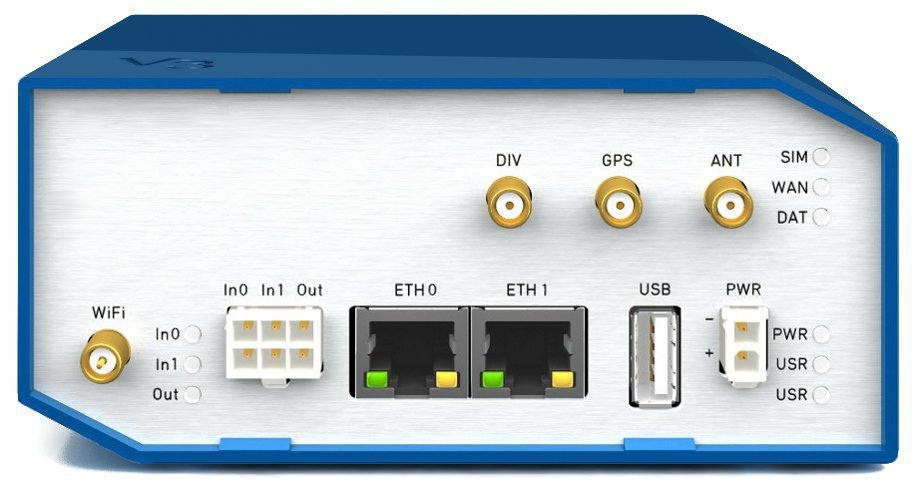
\includegraphics[width=.6\LW]{router}
	\caption{Příklad routeru}
	\label{fig:router}
\end{figure}

Na základě těchto skutečností byl vznešen požadavek na testovací systém. Pomocí tohoto systému bude možné automaticky testovat aktuálně vyvíjený firmware na všech vyráběných modelech routerů a jejich volitelných portech. Zvolena byla kombinace automatizovaného testování a testování založené na modelech. Rozložení těchto dvou způsobů testování bude invidiuální dle testované oblasti či funkcionality. Testování bude pokrývat pouze integrační a systémové testování, jelikož z větší části je firmware do testovaných výrobků tvořen opensource programy. Psaní unit testů pro každý open source program je časově a složitostně nereálné. Systémové testování by mělo probíhat alespoň jednou denně, aby bylo možno případné chyby odchytnout již během vývoje firmwaru a tím usnadnilo a zrychlilo vývoj samotný. Dalším velikým přínosem je zkvalitnění samotného testování, jelikož testovací technici mohou vymýšlet nové testovací procedury a situace namísto opakovaného testování stejných procedur.

\section{Aktuálnost}
Testování každého výrobku před uvedením na trh, či testováním nového firmwaru před jeho vydáním je velmi důležité a nemělo by se opomíjet. Hlavním důvodem je dobré jméno u zákazníka, který nemá zájem o výrobek plný chyb a dále také méně práce pří pozdějším opravování chyb. Při zvyšování počtu výrobků a funkionalit je nutné zvyšovat počet testovacích pracovníků, nebo změnit celý přístup k testování. Jelikož první řešení se zdá být na první pohled neefektivní, tak se v této práci vydám druhou cestou. Při zvyšování efektivity testů použijeme automatizované testování. Dále pokud to bude možné a alespoň trochu efektivní využijeme dnes velmi moderní metodu testování založeného na modelech. Modelovat router jako takový by nejspíše nemělo velký přínos ke zvýšení efektivyty, ale modelování jednotlivých oddělených funkcionalit by mohlo přinést zjednodušení celého testování. V dnešní době birokracie tento systém také pomůže ke schromáždění všech testovacích procedur a reportů ze všech provedených testů na jednom místě.

\section{Výstup práce}
Hlavním cílem práce je hotové řešení automatizovaného systémového řešení testování všech modelů bezdrátových routerů společnosti Conel. Výstupem  řešení bude testovací laboratoř obsahující všechny výrobky, pomocné síťové prvky a testovací server. Dalším výstupem bude aplikace na režii a spouštění testů, interface pro zobrazování reportů ze všech testů s možností administrace testovacího systému. Poslední cíl je vytvoření testovacích procedur pro testování funkcí bezdrátových routerů společnosti Conel.

\section{Struktura práce}
Celou diplomovou práci lze rozdělit do třech částí. V první teoretické částí budou rozebírány všechny různé metody a přístupy k testování samotnému, aby bylo možné dále stavět na teoretickém základu. Dále budou prozkoumány všechny možné dostupné produkty určených k samotnému testování, či produkty sloužící k jednotlivým úkonům potřebným pro otestování daných produktů. Zde bude kladena snaha využít co nejvíce kvalitních hotových řešení sloužícím k účelu testování výrobků společnosti Conel. Ideální cesta by byla nalézt produkt sloužící k našemu účelu, ale jelikož je požadevek velmi specifický, s velkou pravděpodobností bude potřeba z velké části produkt vyvinout. Druhá část se bude zabývat praktickým návrhem všech částí zabývajích se testování každého routeru. Nejdříve bude navrhnuta testovací laboratoř z hlediska všeho potřebného hardwaru. Dále bude popsán návrh a naprogramování programu zajišťující samotné testování a úkony s ním související. Následuje kapitola věnující se uživatelskému interfacu pro reportování výsledků a administraci samotného testování. Samostatná kapitola popisuje api pro zjednodušení psaní testů. Základní api je dodáno s testovacím programem a dále bude popsána možnost dopisování dalších programů. Stěžejní části je kapitola popisující testovací procedury. Poslední částí je praktická implementace testovací laboratoře a testování celého systému. Výstupy z tohoto testování budou použity v poslední kapitole zabývající se možností budoucího vylepšení a rozšíření testovacího systému.

\endinput
